\chapter{Appendix C}
\label{chp:appendixb}

Appendix C contains screenshots and detailed figures from the measurements done in the network built in this thesis. This is meant to be a supplement to the figures presented earlier in the thesis to give the reader a deeper understanding of the system. In addition to the measurements presented here, all data gathered from the system and code used will be public GitHub, \url{http://github.com/sische/MasterThesis}. 

\section{Measured values from tests}

The following two tables present values discussed in chapter 4. These are minimum, average and maximum values of goodput and time between each \gls{coap} packet, using both \gls{con} and \gls{non}. These values have been found by monitoring more than 100 packets in each case. 


\newpage

\begin{table}[H]
\scriptsize
\centering
\caption{Goodput and time, CoAP CON}
\label{goodputTimeCON}
\begin{tabular}{|l|l|l|l|l|l|l|}
\hline
\textbf{Payload} & \textbf{Min goodput} & \textbf{Avg Goodput} & \textbf{Max Goodput} & \textbf{Min Time} & \textbf{Avg Time} & \textbf{Max Time} \\ \hline
0                & 0                    & 0                    & 0                    & 0.27              & 0.28              & 0.35              \\ \hline
50               & 142.41               & 178.12               & 183.09               & 0.27              & 0.28              & 0.35              \\ \hline
100              & 237.56               & 284.8                & 335.87               & 0.3               & 0.42              & 0.35              \\ \hline
150              & 267.9                & 345.33               & 353.34               & 0.41              & 0.44              & 0.56              \\ \hline
200              & 314.52               & 353.53               & 485.6                & 0.41              & 0.57              & 0.64              \\ \hline
250              & 353.74               & 391.43               & 401.35               & 0.62              & 0.64              & 0.71              \\ \hline
300              & 424.29               & 428.58               & 432.81               & 0.69              & 0.7               & 0.71              \\ \hline
350              & 354.35               & 443.3                & 459.17               & 0.76              & 0.79              & 0.99              \\ \hline
400              & 408.16               & 472.34               & 485.63               & 0.82              & 0.85              & 0.98              \\ \hline
450              & 490.37               & 494.4                & 498.64               & 0.9               & 0.91              & 0.92              \\ \hline
500              & 446.23               & 504.35               & 562.4                & 0.89              & 0.99              & 1.12              \\ \hline
550              & 491.24               & 523.1                & 527.21               & 1.04              & 1.05              & 1.12              \\ \hline
600              & 504.16               & 534.45               & 538.85               & 1.11              & 1.12              & 1.19              \\ \hline
650              & 466.14               & 510.67               & 518.67               & 1.25              & 1.27              & 1.39              \\ \hline
700              & 476.04               & 525.06               & 529.18               & 1.32              & 1.33              & 1.47              \\ \hline
750              & 486.82               & 526.31               & 538.33               & 1.39              & 1.43              & 1.54              \\ \hline
800              & 517.42               & 543.6                & 546.74               & 1.46              & 1.47              & 1.54              \\ \hline
850              & 506.12               & 541.44               & 554.19               & 1.53              & 1.57              & 1.68              \\ \hline
900              & 559.14               & 611                  & 615.06               & 1.46              & 1.47              & 1.61              \\ \hline
950              & 502.66               & 559.18               & 567.89               & 1.67              & 1.7               & 1.89              \\ \hline
\end{tabular}
\end{table}



\begin{table}[H]
\scriptsize
\centering
\caption{Goodput and time, CoAP NON}
\label{goodputTimeNON}
\begin{tabular}{|l|l|l|l|l|l|l|}
\hline
\textbf{Payload} & \textbf{Min goodput} & \textbf{Avg Goodput} & \textbf{Max Goodput} & \textbf{Min Time} & \textbf{Avg Time} & \textbf{Max Time} \\ \hline
0                & 0                    & 0                    & 0                    & 0.9               & 1                 & 1.12              \\ \hline
50               & 44.65                & 50.27                & 54.89                & 0.91              & 1                 & 1.12              \\ \hline
100              & 94.6                 & 100.49               & 109.03               & 0.92              & 1                 & 1.06              \\ \hline
150              & 133.93               & 150.66               & 164.85               & 0.91              & 1                 & 1.12              \\ \hline
200              & 117.46               & 201.11               & 221.58               & 0.9               & 1                 & 1.13              \\ \hline
250              & 237.88               & 251.28               & 275                  & 0.91              & 1                 & 1.05              \\ \hline
300              & 252.18               & 302.09               & 357.26               & 0.84              & 1                 & 1.19              \\ \hline
350              & 330.96               & 353.79               & 384.61               & 0.91              & 0.99              & 1.06              \\ \hline
400              & 336.15               & 402.46               & 476.34               & 0.84              & 1                 & 1.19              \\ \hline
450              & 428.41               & 454.6                & 494.93               & 0.91              & 0.99              & 1.05              \\ \hline
500              & 446.52               & 510.38               & 600.09               & 0.83              & 0.98              & 1.12              \\ \hline
550              & 494.21               & 552.72               & 604.61               & 0.91              & 1                 & 1.11              \\ \hline
600              & 570.93               & 607.94               & 613.1                & 0.98              & 0.99              & 1.05              \\ \hline
650              & 531.48               & 568.29               & 580.91               & 1.12              & 1.15              & 1.22              \\ \hline
700              & 543.52               & 577.18               & 591.76               & 1.18              & 1.21              & 1.28              \\ \hline
800              & 553.34               & 585.45               & 601.51               & 1.33              & 1.37              & 1.45              \\ \hline
850              & 556.62               & 591.37               & 609.83               & 1.39              & 1.44              & 1.53              \\ \hline
\end{tabular}
\end{table}


\newpage
The following capture shows a part of a Wireshark capture, as described in chapter \ref{chp:measurements2}.1. This capture shows a \gls{payload} of 0 byte sent using \gls{coap} \gls{non}, and was the base for values used in table \ref{coapCON0table}. 

\begin{figure}[ht]
    \centering
    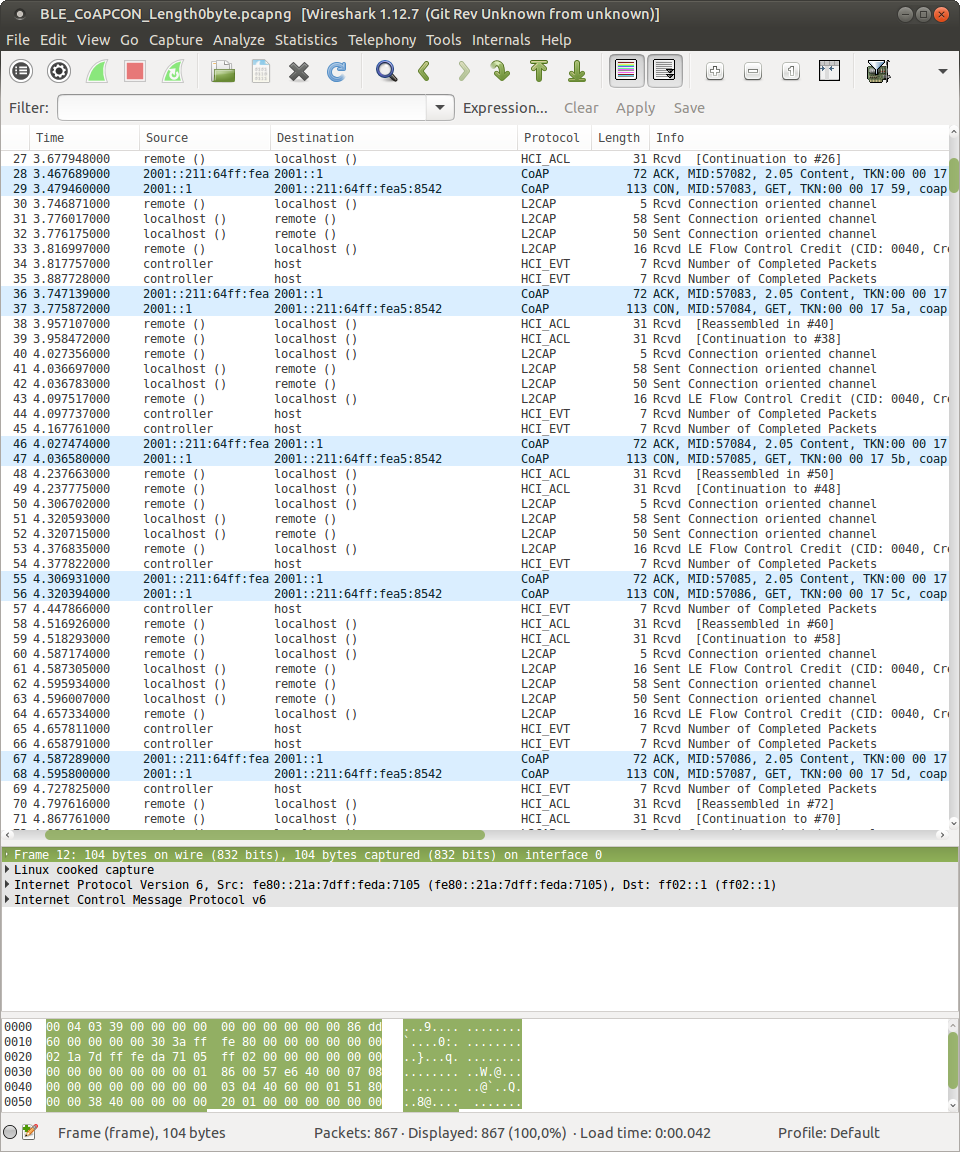
\includegraphics[width=1.0\textwidth]{0byteCONwireshark.png}    
    \caption{Wireshark capture, 0 bytes CON}
    \label{fig:wireshark0byteCONappendixB}
\end{figure}

